\section{Methodology}
 
We define an {\bf event} as a conglomerate of information that encompasses all
of the social media content related to a real-world news occurrence. 
%
Using this specification, which considers an event as a complex unit of
information, we study the type of collective reaction produced by the event on
the social network. 
%
In particular, we analyze the intensity or immediacy of the
social network's response. 
%
By analyzing the levels of intensity in activity induced by different exogenous
events to the network, we are implicitly studying the priority that has been
collectively assigned to the event by groups of independent individuals
\cite{barabasi2005origin, karsai2012universal}. 

We characterize an event's discrete activity dynamics by using
\emph{interarrival times} between consecutive social media messages within an
event (e.g., $d_i = t_{i+1}-t_i$, where $d_i$ denotes the interarrival time
between two consecutive social media messages $i$ and $i+1$ that arrived in
moments $t_i$ and $t_{i+1}$, respectively).


We introduce a novel vectorial representation based on a {\em vector
quantization of the interarrival time distribution}, which we call {\em
``VQ-event model''}. 
%
This model is designed to filter events based on the distribution of the
interarrival times between consecutive messages.  
%
This approach is inspired by the {\em codebook-based representation} from the
field of multimedia content analysis, which has been used in audio processing
and computer vision~\cite{ff,Vaizman}.
%
In our proposed approach, our method learns a set of the most representative
interarrival times from a large training corpus of events; 
%
each one of the representative interarrival times is known as a {\em codeword}
and the complete learned set is known as the {\em codebook}~\cite{Vaizman}. 
%
Each event is then modeled using a vector quantization (VQ) that converts the
interarrival times of an event into a discrete set of values, each value
corresponding to the closest codeword in the codebook \todo{sup}. 
%
The resulting VQ-event model is then a vector in which each dimension contains
the percentage of interarrival times of the event that were assigned a
particular codeword in the codebook.

%%

The VQ-event representation is relative to an event's overall size since the
model is normalized with respect to the number of messages in the event.
%
Therefore the only criteria that are considered in the model are the
interarrival times of each particular event. 
%
This model allows us to group events based on the {\em similarity of the
distribution} of their interarrival times. 
%
In those terms, we consider as high-activity events those events for which the
distribution of interarrival times is most heavily skewed towards the smallest
possible interval, zero. 
%
In other words, events for which the overall activity is extremely intense in
comparison with other events.

%%

To illustrate events with different levels of intensity in activity we present
two examples taken from our analysis of Twitter data. 
%
These examples show the interarrival time histograms for the entire lifecycle of
the two events. 
%
In the first example, the majority of the messages about the death of political
leader Nelson Mandela (Figure~\ref{fig:hi:example-mandela}) arrive within almost
zero seconds of each other. 
%
On the contrary, the messages about The Oscars
(Figure~\ref{fig:hi:example-oscars}) are much more spread out in time.

%%

We note that, by using interarrival times to describe the intensity of the
activity of an event, we make our analysis independent of the particular
evolution of each event. 
%
By doing this, we put no restrictions on how high-activity events unfold in
time, for example, they could be: 
%
(a) events that start out slowly and suddenly gain momentum, 
%
(b) events that go viral soon after they appear on social media and then decay
in intensity over a long (or short) period of time, 
%
(c) events that from the beginning produce large amounts of interest and sustain
that interest throughout their long (or short) lifespan, or 
%
(d) events that are a concatenation of any of the above, etc.






\section{Experimental Analysis}

We study a dataset of news events gathered from news headlines from a
\emph{manually curated} list of well-known news media accounts (e.g., @CNN,
@BreakingNews, @BBCNews, etc.) in the microblogging platform
Twitter~\cite{twitter}. \todo{sup}
%
Headlines were collected periodically every hour, over the course of
approximately one year. 
%
In parallel, all the Twitter messages were extracted for each news event using
the public API \cite{twitterapi}.
%
This process was performed by automatically extracting descriptive sets of
keywords for each event using a variation of frequent itemset
extraction~\cite{Tan_Steinbach_Kumar} over the event's headlines. 
%
These sets of keywords were then used to retrieve corresponding user tweets for
each event. 
%
We validate the events gathered in our data collection process to ensure that
each group of social media posts corresponds to a meaningful and cohesive news
event. 
%
We provide a detailed description of the collection methodology and of
the validation of event cohesiveness in the supplementary material.\todo{sup} 
%
Overall, the resulting dataset contains $43,256,261$ tweets that account for
$5,234$ events (Table~\ref{table:dataset-stats}).


\begin{table}
  \centering
  \begin{tabularx}{\textwidth}{@{}p{6cm}llll@{}}
    \toprule
    \textbf{News events' property} & \textbf{Minimum} & \textbf{Mean} & \textbf{Median} & \textbf{Maximum} \\ \midrule
    \# of posts & 1,000 & 8,254 & 2,474 & 510,920 \\
    \# of keywords & 2 & 3.77 & 3 & 39 \\
    Event duration (hours) & 0.12 & 20.93 & 7.46 & 190.43 \\ \bottomrule
  \end{tabularx}
  \caption{\bf High-level description of the dataset of news events.} 
  \label{table:hi:dataset-stats}
\end{table}



In Figure~\ref{fig:hi:components} we characterize an example event from our
dataset, by showing the set of keywords and a sample of tweets associated to the
event. 
%
These keywords form a semantically meaningful event; they refer to the incident
where soccer player Luis Suarez was charged for biting another player during the
FIFA World Cup in 2014. 
%
This general collection process results in a set of social media posts
associated to an event which can encompass several memes, viral tweets and
pieces of information. 
%
Therefore, an event is composed of diverse information, addressing more
heterogeneous content than prior
work~\cite{Castillo:2014,Szabo:2010,Lerman:2010,Tatar:2011,Pinto:2013,Ahmed:2013,suh2010want}
which focus on single pieces of information (e.g., a particular meme, a viral
tweet etc.).


\begin{figure}
  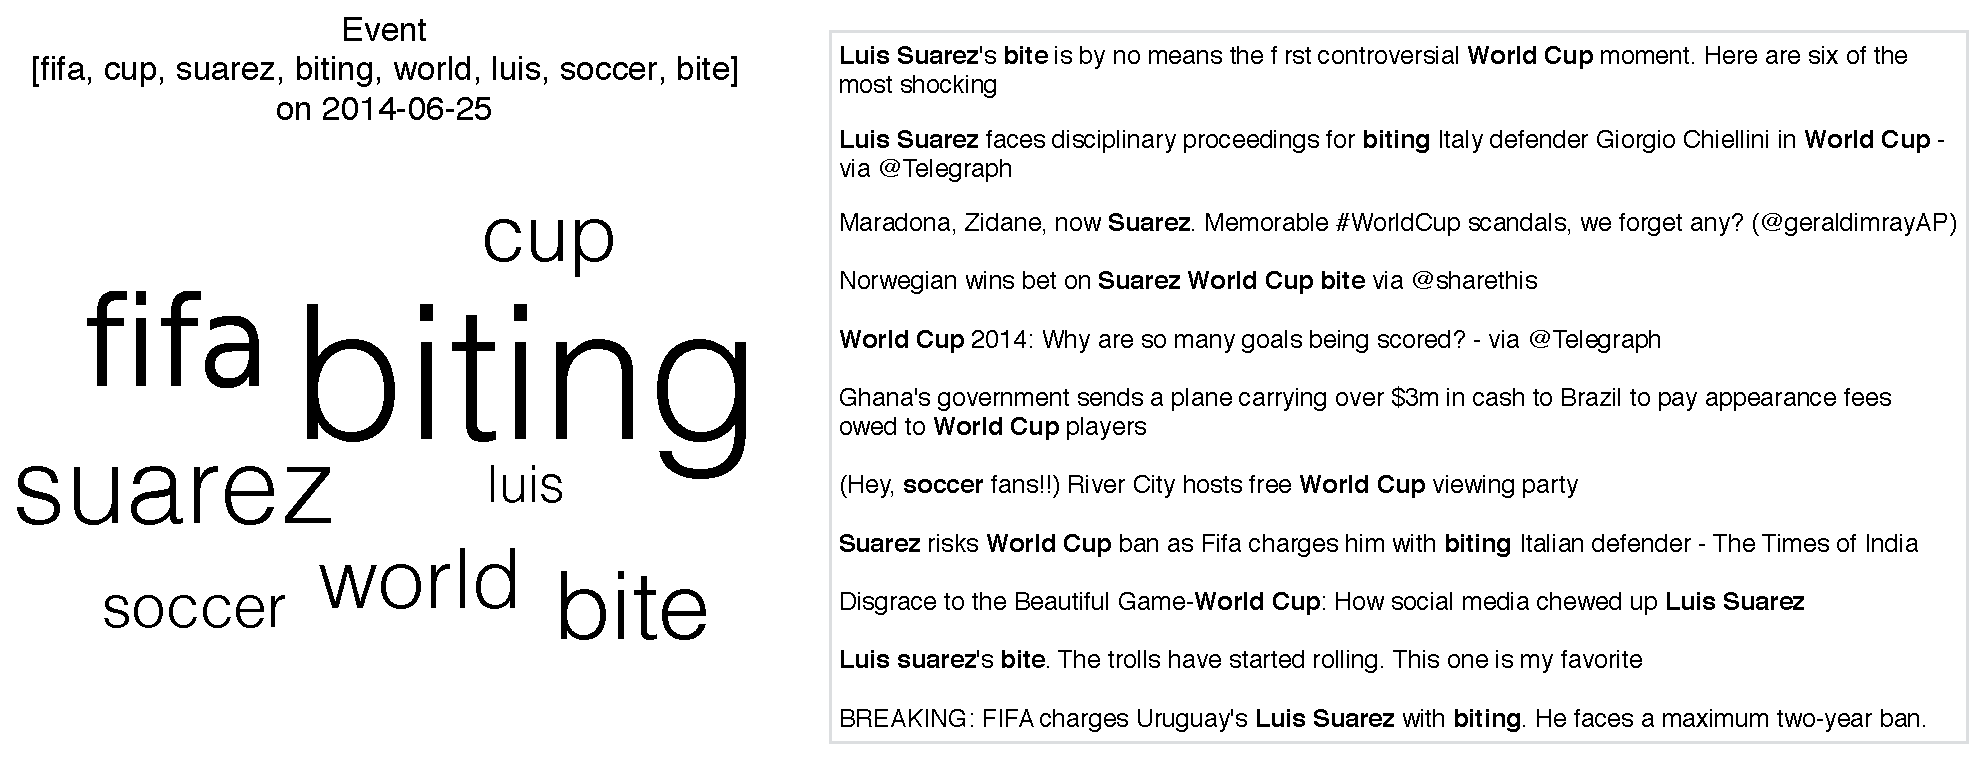
\includegraphics[width=\textwidth]{figures/high-activity/fig2}
  \caption[Example event]{A representative event, collected on 2014-06-25 with
      keywords (left) and sample user posts (right) collected from the Twitter
      Search API. Collected user posts contain at least one pair of keywords. }
  \label{fig:hi:components}
\end{figure}


The collection of events is converted into their VQ-event model representation. 
%
Using this model, we can identify events that have produced similar levels of
activity in the social network. 
%
In other words, events are considered to have similar activity if the
interarrival times between their social media posts are similarly distributed,
implying a very much alike collective reaction from users to the events within a
group. 
%
In order to identify groups of similar events, we cluster the event models. 
%
We sort the resulting groups of events from highest to lowest activity,
according to the concentration of social media posts in the bins that correspond
to short interarrival times. 
%
We consider the events that fall in the top cluster to be high-activity events
as most of their interarrival times are concentrated in the smallest interval of
the VQ-event model.
%
In our dataset, these correspond to roughly 8\% of the events. 
%
We consider the next clusters in the sorted ranking to form medium-high activity
events, and so on. 
%
Thus we end with four groups of events: high, medium-high, medium-low and low.
Figure~\ref{fig:hi:heatmap} shows a heatmap of the interarrival relative
frequency for each cluster. 
%
This classification of events based on activity intensity is independent of
event size. 
%
More details of this methodology are provided in S1 Appendix.
\todo{supp material}

\begin{figure}
  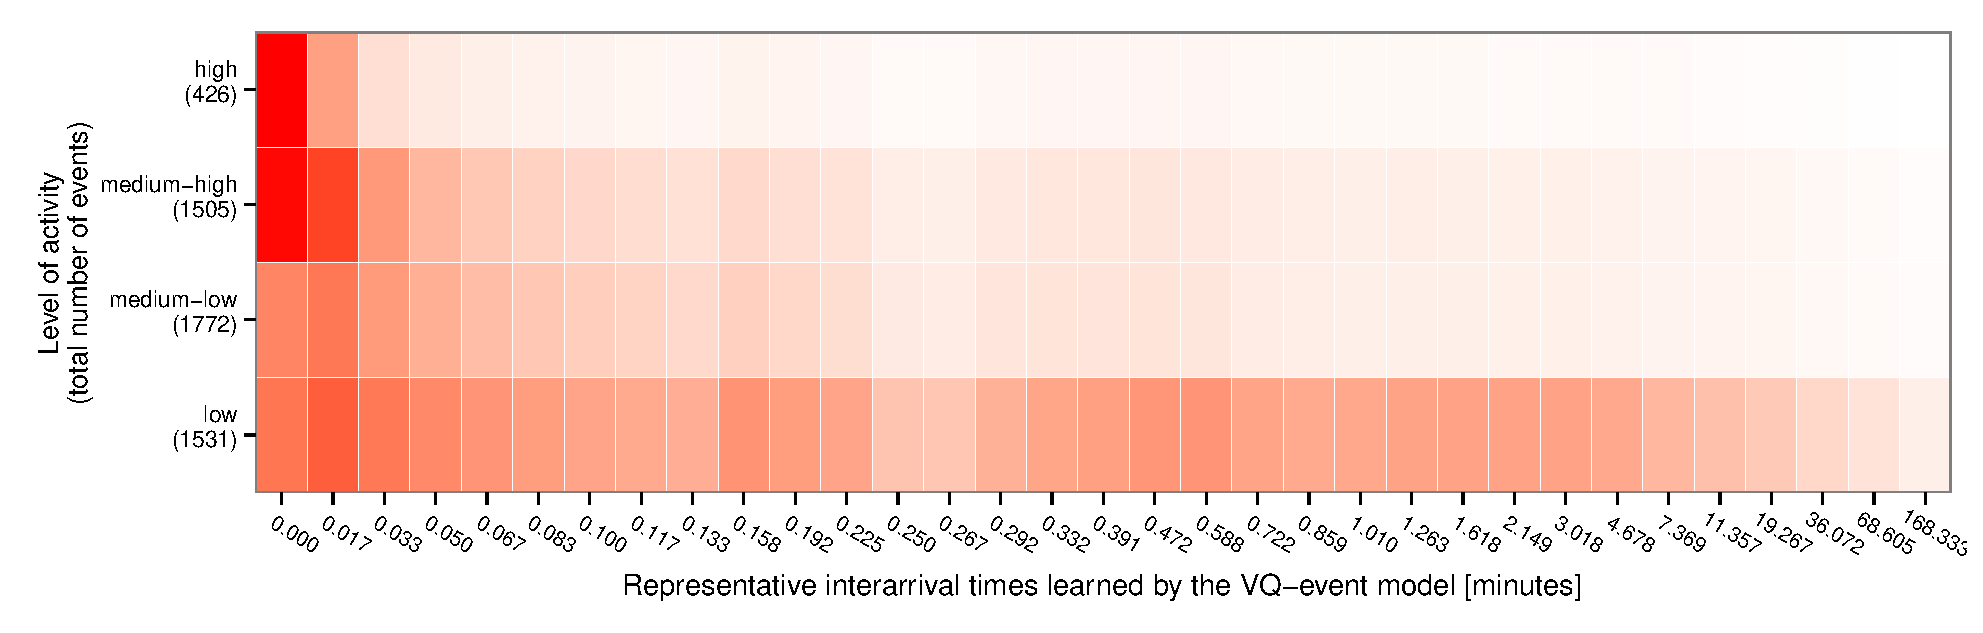
\includegraphics[width=\textwidth]{figures/high-activity/fig3}
  \caption[Heatmap of the categorization of events into clusters of
  activity.]{{Heatmap of the categorization of events into clusters of activity.
  Each row is the average representation of all the events in that clusters.  A
  darker cell represents a higher value. The y-axis specifies the number of
  events in that cluster. Clusters are (top to bottom): high-impact,
  medium-high, medium-low, and low.}}
  \label{fig:hi:heatmap}
\end{figure}